\documentclass[conference]{IEEEtran}
\IEEEoverridecommandlockouts
% The preceding line is only needed to identify funding in the first footnote. If that is unneeded, please comment it out.
\usepackage{cite}
\usepackage{amsmath,amssymb,amsfonts}
\usepackage{algorithmic}
\usepackage{graphicx}
\usepackage{textcomp}
\usepackage{xcolor}
\usepackage{multirow}
\usepackage{hyperref}
\def\BibTeX{{\rm B\kern-.05em{\sc i\kern-.025em b}\kern-.08em
    T\kern-.1667em\lower.7ex\hbox{E}\kern-.125emX}}
\begin{document}

\title{Fall Detection With Motion Tracking
}

\author{\IEEEauthorblockN{Jonathan Edmund Kusnadi}
\IEEEauthorblockA{\textit{Departemen Ilmu Komputer dan Elektronika} \\
\textit{Universitas Gadjah Mada}\\
Sleman, Indonesia \\
jonathan.edmund1202@mail.ugm.ac.id}
}

\maketitle

\begin{abstract}
    Paper ini bertujuan untuk membangun sebuah model Convolutional Neural Network (CNN) yang dapat melakukan klasifikasi gambar X-Ray ke dalam dua kelas yaitu Covid dan Bukan Covid. Dataset yang digunakan adalah http://ugm.id/MVDataset. CNN dipilih karena kemampuannya dalam memproses data gambar yang kompleks. Selain itu, dalam laporan juga disertakan link Google Colab untuk mengakses kode program yang digunakan dalam penelitian. Hasil dari penelitian ini adalah model CNN yang dapat mengklasifikasikan gambar X-Ray ke dalam dua kelas yaitu Covid dan Bukan Covid dengan akurasi 94.5\%.
\end{abstract}

\begin{IEEEkeywords}
COVID-19, Deep Learning, CNN, Detection, Multi-layered CNN, X-Ray
\end{IEEEkeywords}

\section{Introduction}
COVID-19 adalah penyakit pernapasan yang juga mirip dengan influenza.Penyakit ini ditandai dengan batuk kering, sakit kepala, kelelahan, dan demam. Sindrom Distres Pernapasan Akut (ARDS) sering menjadi penyebab kegagalan pernapasan. COVID-19 termasuk dalam Middle East Respiratory Syndrome (MERS). COVID-19 disebabkan oleh betakoronavirus SARS-CoV-2, yang mempengaruhi saluran pernapasan bawah dan menimbulkan pneumonia pada manusia. COVID-19 adalah penyakit yang cukup berbahaya bagi kehidupan manusia, sehingga diperlukan tindakan yang tepat untuk mengurangi dampak pandemi ini. Perubahan-perubahan dibutuhkan dalam sistem kesehatan masyarakat, termasuk diagnostik, penelitian, dan lainnya[1].

Pada saat ini, diagnosis COVID-19 dilakukan dengan menggunakan metode RT-PCR (Reverse Transcription Polymerase Chain Reaction). Metode ini membutuhkan waktu yang cukup lama untuk mendapatkan hasilnya. Selain itu, metode ini juga membutuhkan alat yang cukup mahal. Oleh karena itu, dibutuhkan metode yang lebih cepat dan lebih murah untuk mendeteksi COVID-19. Salah satu metode yang dapat digunakan adalah dengan menggunakan gambar X-Ray. Gambar X-Ray dapat digunakan untuk mendeteksi COVID-19 karena gambar X-Ray dapat menunjukkan adanya pneumonia pada paru-paru[1].

Deep learning merupakan salah satu teknik dalam machine learning yang menggunakan model neural network dengan banyak layer untuk mempelajari fitur-fitur yang kompleks dari data dan melakukan prediksi atau klasifikasi dengan akurasi yang tinggi. Salah satu jenis neural network yang populer dalam deep learning adalah convolutional neural network (CNN)[1].

Menurut sebuah paper, CNN merupakan jenis neural network yang dirancang khusus untuk mengolah data dengan struktur grid atau matriks, seperti gambar[2]. CNN menggunakan konvolusi untuk mempelajari fitur-fitur pada data dan pooling untuk mengurangi dimensi data, sehingga mampu menangani input yang besar dan kompleks.

CNN banyak digunakan dalam berbagai aplikasi seperti pengenalan wajah, pengenalan tulisan tangan, klasifikasi gambar, dan lain sebagainya. Keunggulan dari CNN adalah kemampuannya untuk mempelajari fitur-fitur dari data secara otomatis, tanpa perlu fitur ekstraksi manual. Hal ini membuat CNN menjadi sangat efektif dan efisien dalam mengolah data yang kompleks.

Pada penelitian ini, CNN digunakan untuk mengklasifikasikan gambar X-Ray ke dalam dua kelas yaitu kelas yang terdiagnosis dengan Covid-19 dan kelas yang normal. Penelitian ini bertujuan untuk mencari model CNN yang optimal untuk deteksi atau diagnosis Covid-19.

\section{Methodology}

\subsection{Dataset}
Pada penelitian ini awalnya menggunakan dataset yang digunakan adalah dataset dari Joseph Paul Cohen, Paul Morrison dan Lan Dao yang berisi 156 gambar X-Ray paru-paru. Namun untuk membangun model CNN yang lebih baik, dataset tersebut ditambahkan dengan dataset dari Muhammad E. H. Chowdhury et al. yang berisi 13964 gambar[3][4]. Namun dataset tersebut memiliki kelas yang tidak seimbang sehingga dilakukan proses undersampling untuk mendapatkan dataset yang seimbang. Dataset yang digunakan pada penelitian ini adalah dataset yang sudah dilakukan undersampling sehingga dataset yang digunakan memiliki jumlah 8819 gambar dengan distribusi data pada Fig 1 dan sampel dari dataset pada Fig 2 dan Fig 3.

\begin{figure}[htbp]
    \centerline{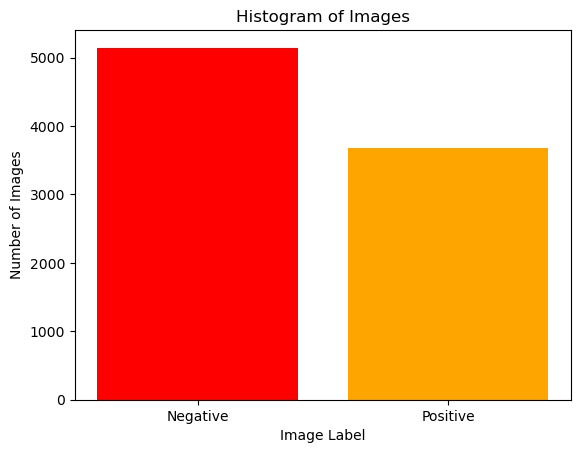
\includegraphics[width=0.5\textwidth]{figures/distribusi_dataset_final.png}}
    \caption{Distribusi kelas pada dataset}
\end{figure}
\begin{figure}[htbp]
    \centerline{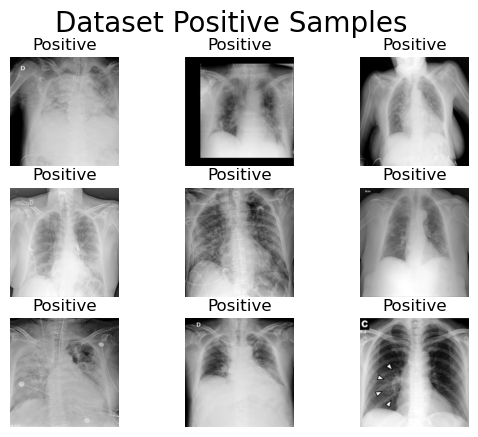
\includegraphics[width=0.5\textwidth]{figures/positive_samples.png}}
    \caption{Sampel positif dataset}
\end{figure}
\begin{figure}[htbp]
    \centerline{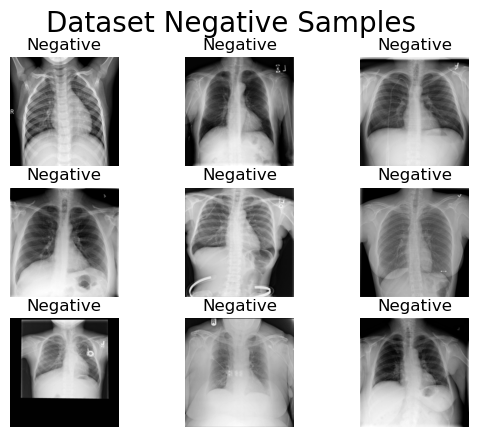
\includegraphics[width=0.5\textwidth]{figures/negative_samples.png}}
    \caption{Sampel negatif dataset}
\end{figure}
Dataset kemudian di pisah menjadi tiga bagian yaitu training set, validation set, dan test set. Training set dan validation set digunakan untuk melatih model CNN, sedangkan test set digunakan untuk mengevaluasi performa dari model CNN. Training set sejumlah 60\% dari dataset, validation set sejumlah 20\% dari dataset, dan test set sejumlah 20\% dari dataset.

\subsection{Preprocessing}
Pada tahap preprocessing, gambar-gambar pada dataset diubah ukurannya agar seragam. Gambar-gambar pada dataset juga diubah menjadi grayscale karena gambar X-Ray pada dataset tersebut masih dalam bentuk RGB. Gambar-gambar pada dataset juga di normalisasi dengan membagi setiap pixel dengan 255. Hal ini dilakukan untuk mengurangi waktu yang dibutuhkan untuk melatih model CNN.

Normalisasi pada gambar (image normalization) sangat penting untuk dilakukan dalam pelatihan model Convolutional Neural Network (CNN) karena dapat meningkatkan performa model dengan mengurangi variabilitas dalam data masukan. Menurut literatur, normalisasi pada gambar dalam CNN dapat didefinisikan sebagai \textit{"the process of transforming input images so that they have similar statistical properties, which can improve the performance of the model"} [5].

\subsection{CNN Architecture}
Arsitektur dari model CNN yang diusulkan terdiri dari lima belas lapisan. Arsitektur diawali dengan lapisan konvolusi dua dimensi dengan input gambar 200 x 200 piksel yang kemudian dilanjutkan dengan lapisan \textit{max pooling}. Kemudian dilanjutkan dengan lapisan konvolusi, lapisan normalisasi, dan \textit{max pooling}, ketiga lapisan tersebut diulang sebanyak tiga kali. Hasil kemudian di \textit{flatten} dan dimasukan dalam dua lapisan \textit{dense} atau \textit{neural network} yang memiliki 128 \textit{neuron}. Kemudian dilanjutkan dengan lapisan \textit{dropout} yaitu penghapusan neuron secara random sebagai upaya untuk memperkecil kemungkinan \textit{overfitting}. Lapisan \textit{dropout} diikuti dengan lapisan \textit{dense} yang memiliki satu \textit{neuron} yang merupakan output dari model CNN. Arsitektur dari model CNN dapat dilihat pada Fig 3.

\begin{figure}[htbp]
    \centerline{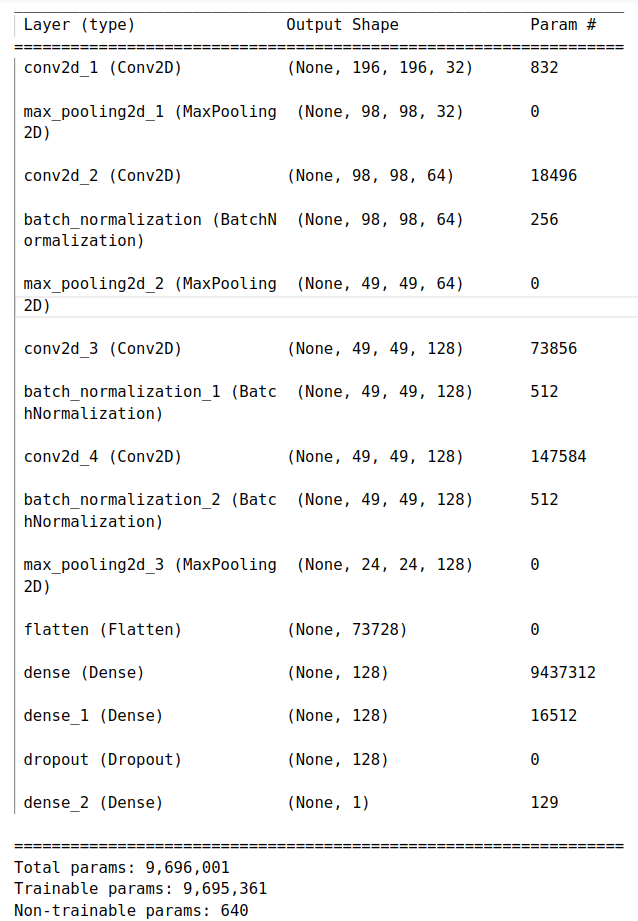
\includegraphics[width=0.5\textwidth]{figures/cnn_layers.png}}
    \caption{Arsitektur model CNN}
\end{figure}

Parameter yang digunakan pada model CNN adalah sebagai berikut:
\begin{itemize}
    \item \textbf{Optimizer}: Adam
    \item \textbf{Learning rate}: 0.001
    \item \textbf{Loss function}: Binary Crossentropy
    \item \textbf{Batch size}: 32
    \item \textbf{Epoch}: 50
\end{itemize}
Untuk mengoptimalkan efisiensi dari tahap pelatihan model CNN, digunakan beberapa \textit{callback} yaitu \textit{early stopping} dan \textit{ReduceLROnPlateau}. 

\begin{itemize}
    \item \textbf{Early Stopping} \\
    \textit{Early stopping} digunakan untuk menghentikan proses pelatihan model CNN ketika model sudah tidak mengalami peningkatan performa dalam 5 epoch. Callback Early Stopping adalah teknik yang digunakan dalam pelatihan model Convolutional Neural Network (CNN) untuk menghentikan pelatihan saat performa model tidak lagi meningkat. Teknik ini membantu mencegah overfitting dan mempercepat proses pelatihan. Menurut literatur, callback early stopping pada CNN dapat didefinisikan sebagai \textit{``a technique in deep learning that monitors the validation loss of a CNN model during training and stops the training process when the validation loss no longer improves over a certain number of epochs''} [6].\\

    \item \textbf{ReduceLROnPlateau} \\
    \textit{ReduceLROnPlateau} adalah teknik yang digunakan dalam pelatihan model Convolutional Neural Network (CNN) untuk menurunkan laju belajar (learning rate) saat performa model tidak lagi meningkat. Teknik ini membantu mencegah terjebak di dalam lokal minimum dan mempercepat proses konvergensi. Menurut literatur, callback ReduceLROnPlateau pada CNN dapat didefinisikan sebagai \textit{"a callback function in deep learning that monitors the validation loss of a CNN model during training and reduces the learning rate of the optimizer when the validation loss stops improving for a certain number of epochs"} [7].
\end{itemize}
Parameter yang digunakan pada \textit{callback} yang digunakan tertera dalam Table 1.

\begin{table}[htbp]
    \begin{center}
    \caption{Callback Parameter}
    \begin{tabular}{|l|l|l|}
    \hline
    \textbf{Callback} & \textbf{Parameter} & \textbf{Value} \\
    \hline
    \multirow{3}{*}{Early Stopping} & min\_delta & 0.01 \\ \cline{2-3} 
                                    & patience & 10 \\ \cline{2-3} 
                                    & restore\_best\_weights & True \\ \hline
    \multirow{3}{*}{ReduceLROnPlateau}  & factor & 0.1 \\ \cline{2-3} 
                                        & patience & 5 \\ \cline{2-3} 
                                        & min\_delta & 0.01 \\ \hline
    \end{tabular}
    \end{center}
    \end{table}

\section{Results and Discussion}
Pada penelitian ini, digunakan perangkat komputasi GPU NVIDIA GeForce GTX 1650. Pelatihan model selesai pada epoch ke-27 disebabkan \textit{callback early stopping}. Grafik \textit{loss} dan akurasi dari model CNN dapat dilihat pada Fig 5 dan Fig 6.

\begin{figure}[htbp]
    \centerline{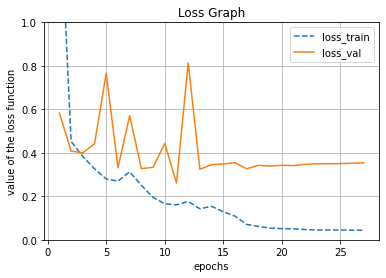
\includegraphics[width=0.5\textwidth]{figures/loss.png}}
    \caption{Grafik \textit{loss} dari model CNN}
\end{figure}

\begin{figure}[htbp]
    \centerline{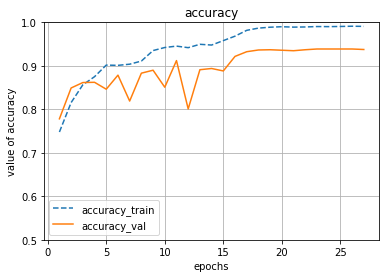
\includegraphics[width=0.5\textwidth]{figures/accuracy.png}}
    \caption{Grafik akurasi dari model CNN}
\end{figure}

Grafik \textit{loss} menunjukan bahwa model CNN yang diusulkan memiliki \textit{loss} yang semakin menurun seiring dengan bertambahnya epoch walaupun terjadi fluktuasi yang signifikan pada awal. Hal tersebut menunjukkan bahwa model CNN yang diusulkan semakin baik dalam melakukan klasifikasi gambar X-ray paru-paru.

Grafik akurasi menunjukkan bahwa model CNN yang diusulkan memiliki akurasi yang semakin meningkat seiring dengan bertambahnya epoch. Hal tersebut menunjukkan bahwa model CNN yang diusulkan semakin baik dalam melakukan klasifikasi gambar X-ray paru-paru.

Dari hasil pelatihan model CNN, didapatkan akurasi sebesar 94\% dan \textit{loss} sebesar 23\%. Hasil tersebut menunjukkan bahwa model CNN yang diusulkan memiliki performa yang baik dalam melakukan klasifikasi gambar.

\section{Conclusion}
Pada penelitian ini, model Convolutional Neural Network (CNN) terbukti dapat melakukan klasifikasi Covid-19 berdasarkan gambar X-ray paru-paru. Model CNN yang diusulkan memiliki akurasi sebesar 94\% dan \textit{loss} sebesar 23\%. Hasil tersebut menunjukkan bahwa model CNN yang diusulkan memiliki performa yang baik dalam melakukan klasifikasi gambar X-ray paru-paru. 

Untuk penelitian selanjutnya, dapat dilakukan penelitian dengan menggunakan dataset yang lebih besar dan beragam. Selain itu, dapat dilakukan penelitian dengan melakukan pengolahan citra seperti \textit{histogram equalization} beserta metode \textit{preprocessing} lainnya pada dataset. Untuk menghasilkan akurasi yang lebih tinggi, dapat dilakukan penelitian dengan menggunakan model CNN yang lebih kompleks seperti ResNet, DenseNet, dan EfficientNet. Dapat juga dilakukan penelitian dengan menggunakan \textit{transfer learning} untuk meningkatkan akurasi dari model CNN yang diusulkan.

\section{Additional Information}
File \textit{Google Colab} atau \textit{Jupyter Notebook} dapat diakses pada tautan berikut: \url{https://colab.research.google.com/drive/1dv7vCyRvFQis5hKDv8Sr2cJx3V8V1lo5}

\begin{thebibliography}{00}
\bibitem{b1} A. S. N. Zainab, I. Soesanti and D. R. Utomo, "Detection of COVID-19 using CNN's Deep Learning Method: Review," 2022 4th International Conference on Biomedical Engineering (IBIOMED), Yogyakarta, Indonesia, 2022, pp. 59-64, doi: 10.1109/IBIOMED56408.2022.9988533.
\bibitem{b2} Y. LeCun, Y. Bengio and G. Hinton, "Deep learning," in Nature, vol. 521, no. 7553, pp. 436-444, May 2015, doi: 10.1038/nature14539.
\bibitem{b3} M.E.H. Chowdhury, T. Rahman, A. Khandakar, R. Mazhar, M.A. Kadir, Z.B. Mahbub, K.R. Islam, M.S. Khan, A. Iqbal, N. Al-Emadi, M.B.I. Reaz, M. T. Islam, “Can AI help in screening Viral and COVID-19 pneumonia?” IEEE Access, Vol. 8, 2020, pp. 132665 - 132676. Paper link
\bibitem{b4} Rahman, T., Khandakar, A., Qiblawey, Y., Tahir, A., Kiranyaz, S., Kashem, S.B.A., Islam, M.T., Maadeed, S.A., Zughaier, S.M., Khan, M.S. and Chowdhury, M.E., 2020. Exploring the Effect of Image Enhancement Techniques on COVID-19 Detection using Chest X-ray Images. Paper Link
\bibitem{b5} Y. Chen, Z. Shi, B. Zhou, and J. Zhu, "Deep Learning for Computer Vision: Theory, Algorithms, and Applications," Springer, 2019, pp. 103-105.
\bibitem{b6} Y. Chen, Z. Shi, B. Zhou, and J. Zhu, "Deep Learning for Computer Vision: Theory, Algorithms, and Applications," Springer, 2019, pp. 153-154.
\bibitem{b7} S. Huang, "Deep Learning for Image Recognition," CRC Press, 2019, pp. 133-134.
\end{thebibliography}

\end{document}